\section{Challenges and beyond near future} \label{challenges}

%%%%%%%%%%%%%%%%%%% sensing on the small and cheap and computing goes mainstream


As discussed, the field of software defect prediction has made many accomplishments in the recent years. However, many challenges remain and will pop up in the future do to changes in technology, data and the increasingly important role software systems continue to play.

%%%%%%%%%%%%%%%%%%%%%%%%%%%%%%%%%%%%%%%%%%%%%%%%%%%%%%%%%%%
\subsection{Data collection}
\smallsection{Future Challenge 1: Commercial vs. OSS Data}
As Section \ref{trends} shows, many researchers make use of the dataset collected from open source software projects. The main reason for using data from open source projects is that these projects archive long and practical development history and make their data publicly available. However, the generality of our findings and techniques to non open source software projects (e.g., commercial projects) is not studied in depth; in part due to the lack of availability of data. 
%The challenge is that the number of public industrial datasets is limited (e.g., only NASA datasets).

To solve this challenge, we need to make more partnership with industrial partners and have access to their repositories. The authors had some success starting projects with industry and our experience shows that starting such partnerships is easier than one might think. Especially with the hype of big data and data analysis in general, companies tend to realize that there is value in mining their data. That said, the industrial partners need to see some value with what the researchers are doing with their data, otherwise they may lose interest.

Many industrial projects have already shifted to modern software development environment (e.g., Git and Gerrit). That is, it is easy to apply our tool to their projects. Practitioners are also curious about knowing their quality using MSR techniques. 
In short, the most important thing is to have the will to start a collaboration with industrial projects. when we continue to demonstrate the value of data in software repositories and the benefits of MSR techniques for helping practitioners in their daily activities, practitioners are more likely to contact us and consider using our technique in practice. 

\begin{comment}
\smallsection{Challenge 2 (beyond near future): Reactive vs. Proactive}
When it comes to software defect prediction, many of our techniques thus far have been reactive in nature. What that means is that we observe the software development process and then use this data to predict what will happen post-release. However, in many cases practitioners would like to have predictions happen much sooner, e.g., before or as soon as they commit their changes. Doing so would make our approaches more proactive in a sense, since it will allow us to perform our predictions as the development is happening rather than waiting till it has completed.

Several studies have already started to work in this area, using metrics from the design stage \todo{cite Zeller's paper} and performing change-level defect predictions \todo{cite JIT}. However, there remains much work to do in this area. We maybe able to devise tools that not only predict risky areas or changes, but also generate tests (and possibly fixes) for these risky areas and changes. We can also devise techniques that proactively warn developers, even before they modify the code, that they are working with risky code that has had specific types of defects in the past.


Currently, we feel that we are likely to be reactive to repositories. We try to find and use the repositories that are valuable and not much studied for our studies. For example, GitHub, which is a Web-based Git repository hosting service, started in 2008, then was becoming very well-known and frequently-used Git repository hosting service around 2009-2010. Several studies~\cite{Ray2014FSE} conduct a large scale empirical studies of defect prediction by making use of the dataset collected from a pile of projects on GitHub. \emad{Yasu, I am not sure about what you wrote here man!}

We do not mention that we throw in seeking the repositories that are not much studied. The data needed to perform defect prediction is readily available as it is collected by projects for other purposes. Therefore, practitioners do not have to spend additional effort in their projects.

However, if we are proactive to repositories, we may be able to go forward into the next stage of defect prediction studies. We could propose the tool that not only archives the data needed to perform defect prediction, but also helps practitioners' daily decision-processes in modern software development organizations. Such tool (e.g., Mylyn~\cite{Lee2011FSE}) does not force them to spend additional effort in their projects. 
\end{comment}

%The feedbacks from users to software systems are valuable and fundamental for improving software quality. 

\begin{comment}
\smallsection{Developer feedbacks: Stack Overflow}
Developer feedbacks can be used for knowing how developers solve defects and 

\para{StackOverflow}
\yasu{Do you know any papers that use the data collected from StackOverflow?}
\url{here is a link: http://meta.stackexchange.com/questions/134495/academic-papers-using-stack-exchange-data/134496#134496}
\end{comment}

%%%%%%%%%%%%%%%%%%%%%%%%%%%%%%%%%%%%%%%%%%%%%%%%%%%%%%%%%%%
\subsection{Metrics calculation}

\smallsection{Future Challenge 2: Considering New Market}
The majority of software defect prediction studies used code and/or process metrics to perform their predictions. To date, this has served the community well and has helped us advance the state-of-the-art in software defect prediction.
However, comparing with year 2000, our environment has changed dramatically. Therefore, we need to tackle the defects that new environments raise. 

One example of a new market that we should tackle is mobile application fields. We use personal smart phone every day during moving and update applications from online stores (e.g., Google Play and App Store). Mobile applications play a significant role in our daily life and these applications have different characteristics compared to conventional applications that we studied in the past. These mobile application stores allow us to gain valuable user data that, till today, has not been leveraged in the area of software defect prediction. Few studies have leveraged this data to improve testing \cite{Khalid2014FSE,Khalid2015IEEESoft}. Moreover this data can be leveraged to help us understand what impacts users and in which way the user is impacted. Such knowledge can help us build better and more accurate models. We anticipate the use of user data in software defect prediction models to be an area of significant growth in the future.

Energy consumption has been one of the greatest challenge for software industries in the coming decade. Software systems are currently hosted on more than 35 million servers across thousands of data centers. Hindel published papers~\cite{Hindle2012ICSE,Hindle2012MSR} related to energy consumption (green mining) in SE conferences in 2012, then the green mining are now one of the hottest topics in SE domain~\cite{Pinto2014MSR,Sahin2014ICSME}. For future, we should develop some metrics and modeling techniques for energy consumption.

\begin{comment}
\yasu{Emad: I dropped the below, because it seems not to fit}
The fact is, research moves at a very fast speed, which is too fast for any one researcher or group. It is difficult for the one person/group to understand the problem of the modern techniques in other market fields. 
Collaborating with others from other domains can help us advance the field in a novel and speedy way. There are some good examples where collaborations with the researchers across domains have succeeded. For example, one paper~\cite{Nam2013ICSE} is published with SE researchers (1st and 3rd authors) and a data mining researcher (2nd author). The paper first applied TCA \emad{need to expand this}, which was proposed by the 2nd author and tried to reduce the data distribution difference between training and testing data, to defect prediction. However, they found that the performance of cross-project defect prediction with TCA is sensitive to normalization. Therefore, they proposed a novel transfer defect learning approach, TCA+, by extending TCA. We also find other examples where collaborations between SE researchers and natural language processing have been fruitful~\cite{Oda2015ASE}.
\end{comment}

\begin{comment}
\smallsection{Challenge 6: Getting more accurate models}
\emad{Yasu, this section is a little strange. I am not sure what you want to say here man! We already have pretty accurate models. I think we should say here that we need to be more accurate at detecting impactful bugs and build models that people can understand.}
One of the challenges is that we develop the models that always provide high accurate defect prediction models (i.e., high precision and recall).
Craig Federighi, who is Apple's senior vice president of software engineering, said the speech recognition capability in Siri now has a 5 percent word error rate, thanks to a 40 percent reduction on the part of Apple at Apple's 2015 Worldwide Developers Conference~\cite{}. While such high accurate recognition would keep the motivation of what people want to use Siri, low accurate one loses the motivation. It happens for defect prediction models. Low accurate models waste the time of developers, then developers lose the interest of the models and do not believe the alarm of the defect prediction models like \emph{The Boy Who Cried Wolf}. It is a big challenge to get 5 percent error rate for defect prediction models for future.
\end{comment}

\begin{comment}
\smallsection{Challenge 4: Collaborating with other domain researchers}
We often make use of techniques that are proposed in other research fields (e.g., data mining and AI) to build better defect prediction models~\cite{Breiman2001}. Many modern techniques are available via packages in R and Weka (e.g., Random Forest and Latent Dirichlet allocation). 
However, such techniques are sometimes not suitable for software engineering datasets due to uniqueness of SE data (e.g., the number of defect-inducing changes represents only a tiny percentage of all changes).

The fact is, research moves at a very fast speed, which is too fast for any one researcher or group. It is difficult for the one person/group to understand the problem of the modern techniques in other research fields and revise and apply them to defect prediction studies. We are likely to have more knowledge about dataset in the SE research field and how to use statistical/machine learning packages, but less mathematical knowledge to re-implement the modern techniques.

Collaborating with others from other domains can help us advance the field in a novel and speedy way. That said, it is challenging to collaborate , because we have less chance to meet the researchers in other research domain than the researchers in same domain and need to raise the research goal that both researchers are interested in.

There are some good examples where collaborations with the researchers across domains have succeeded. For example, one paper~\cite{Nam2013ICSE} is published with SE researchers (1st and 3rd authors) and a data mining researcher (2nd author). The paper first applied TCA \emad{need to expand this}, which was proposed by the 2nd author and tried to reduce the data distribution difference between training and testing data, to defect prediction. However, they found that the performance of cross-project defect prediction with TCA is sensitive to normalization. Therefore, they proposed a novel transfer defect learning approach, TCA+, by extending TCA. We also find other examples where collaborations between SE researchers and natural language processing have been fruitful~\cite{Oda2015ASE}.

In short, collaborating with the researchers in other research domains will not only help us use modern techniques, but also extend them to fit our research domain.
\end{comment}

%%%%%%%%%%%%%%%%%%%%%%%%%%%%%%%%%%%%%%%%%%%%%%%%%%%%%%%%%%%
\subsection{Model building}

\smallsection{Future Challenge 3: Moving Fast!} 
In today's fast changing business environment, the recent trend of software development is to reduce the release cycle to days or even hours~\cite{RELENG2015}.
For example, the Firefox project changes their release process to a rapid release model (i.e., a development model with a shorter release cycle) and releases over 1,000 improvements and performance enhancements with version 5.0 in 3 months~\cite{Khomh2015EMSE}.
IMVU, which is an online social entertainment website, deploys new code fifty times a day on average ~\cite{AdamsICSE2012}.

We need to think about how we integrate our research into contentious integration.
For example, O'Hearn suggested that commenting on code changes at review time makes a huge difference in helping developers than producing the bug list from batch-mode analysis because such commenting does not ask them to make a context switch to understand and act on an analysis report~\cite{CAV2015}.

The majority of quality assurance research focused on defect prediction models that identify defect-prone modules (i.e., files or packages) at release-level like batch-mode analysis~\cite{Gyimothy2005,hassan2009,Li2006,Munson1992}. Those studies use the dataset collected from previous release to build a model and derive the bug list that includes the probability of defect prone of all modules. Such model require practitioners to remember the rationale and all the design decisions of the change to be able to evaluate if the change introduced a defect.

To solve the problem that O'Hearn pointed out, we can focus on Just-In-Time (JIT) Quality Assurance~\cite{kamei2013tse,Mockus2000BTJ,Kim2008TSE}, which performs predictions at the change level. JIT defect prediction models aim to be an earlier step of continuous quality control because it can be invoked as soon as a developer commits code to their private or to the team’s workspace.

There remains much work to do in this area. As future challenge, we still need to evaluate how to integrate JIT models into actual contentious integration process. For example, we can devise the approaches that suggest how many effort developers spend to find and fix defects based on the probability of prediction (e.g., while JIT models predict that this change includes defects with 80\% of probability, the developer should work on the change for additional 30 minutes to find the defects). 
We are also maybe able to devise tools that not only predict risky areas or changes, but also generate tests (and possibly fixes) for these risky areas and changes. We can also devise techniques that proactively warn developers, even before they modify the code, that they are working with risky code that has had specific types of defects in the past.

%\para{Peter  says ``Moving fast!'' batch-mode analysis => just-in-time mode analysis}

%-----------------------------------------------------------------------
\begin{figure}
  \centering
  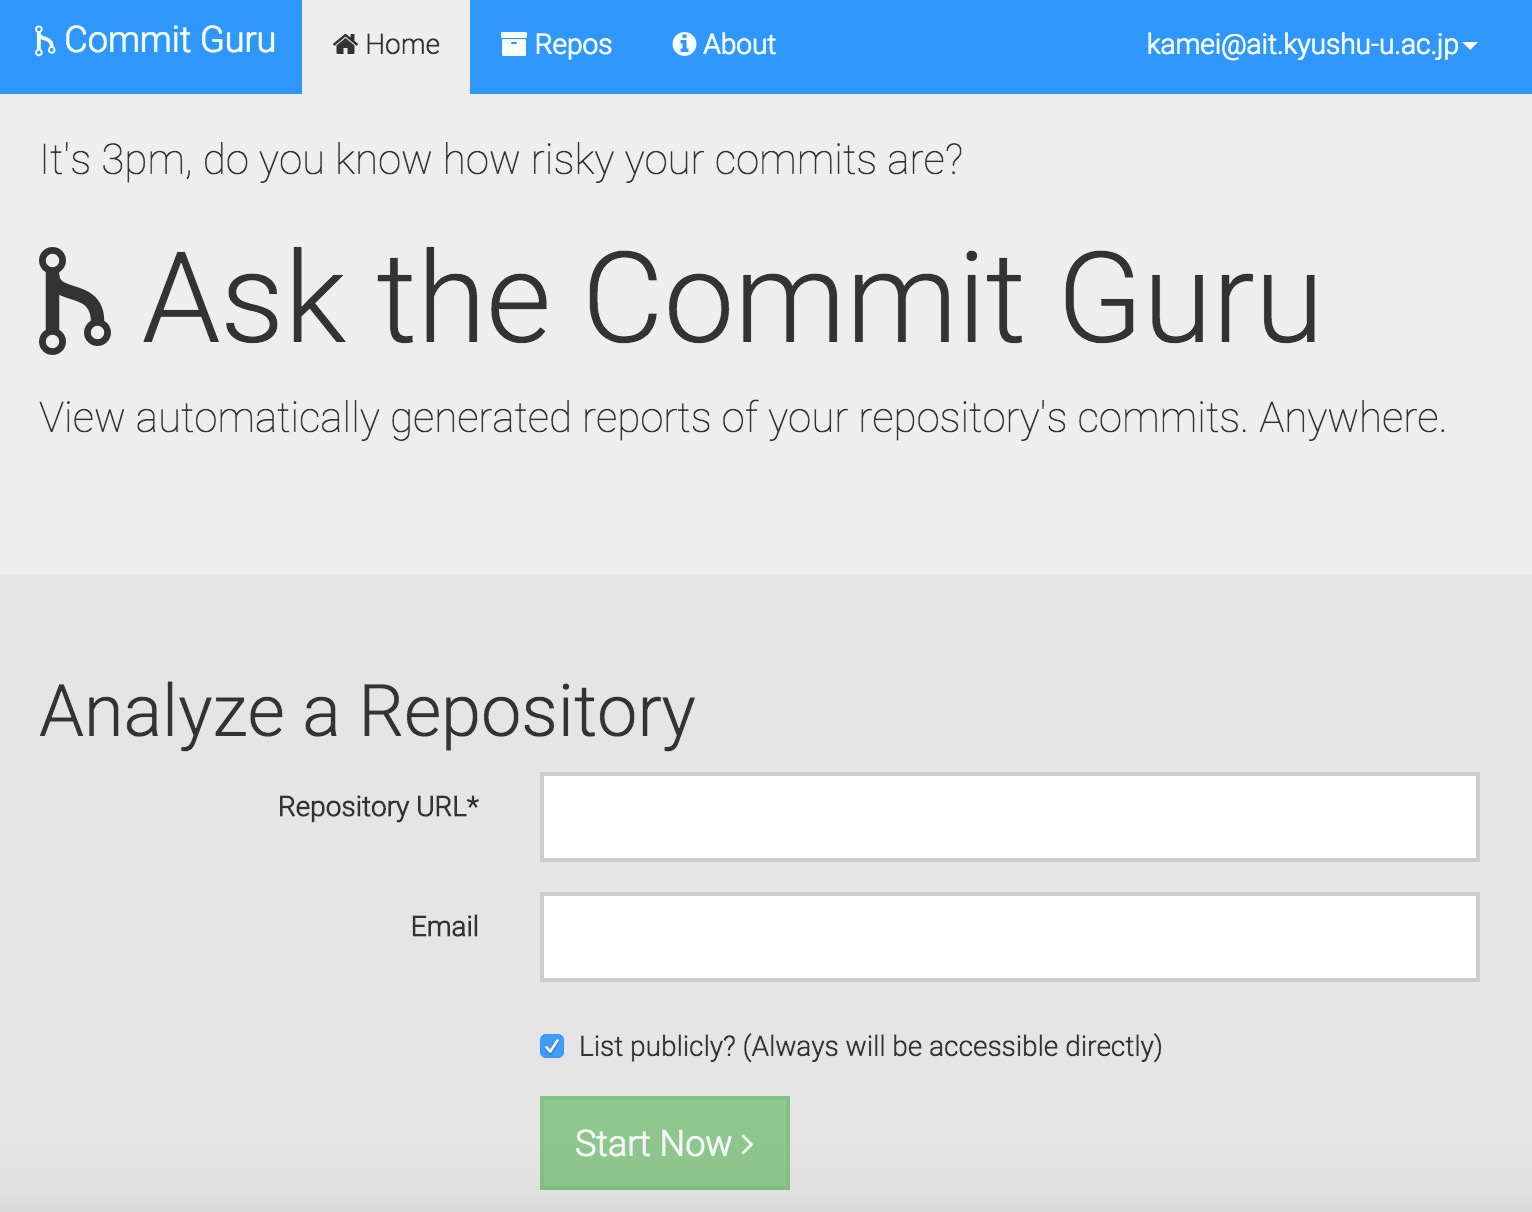
\includegraphics[width=.4\textwidth]{figures/guru1}
  \caption{Adding a Repository in Commit Guru \label{fig:guru1}}
\end{figure}
%-----------------------------------------------------------------------

%-----------------------------------------------------------------------
\begin{figure}
  \centering
  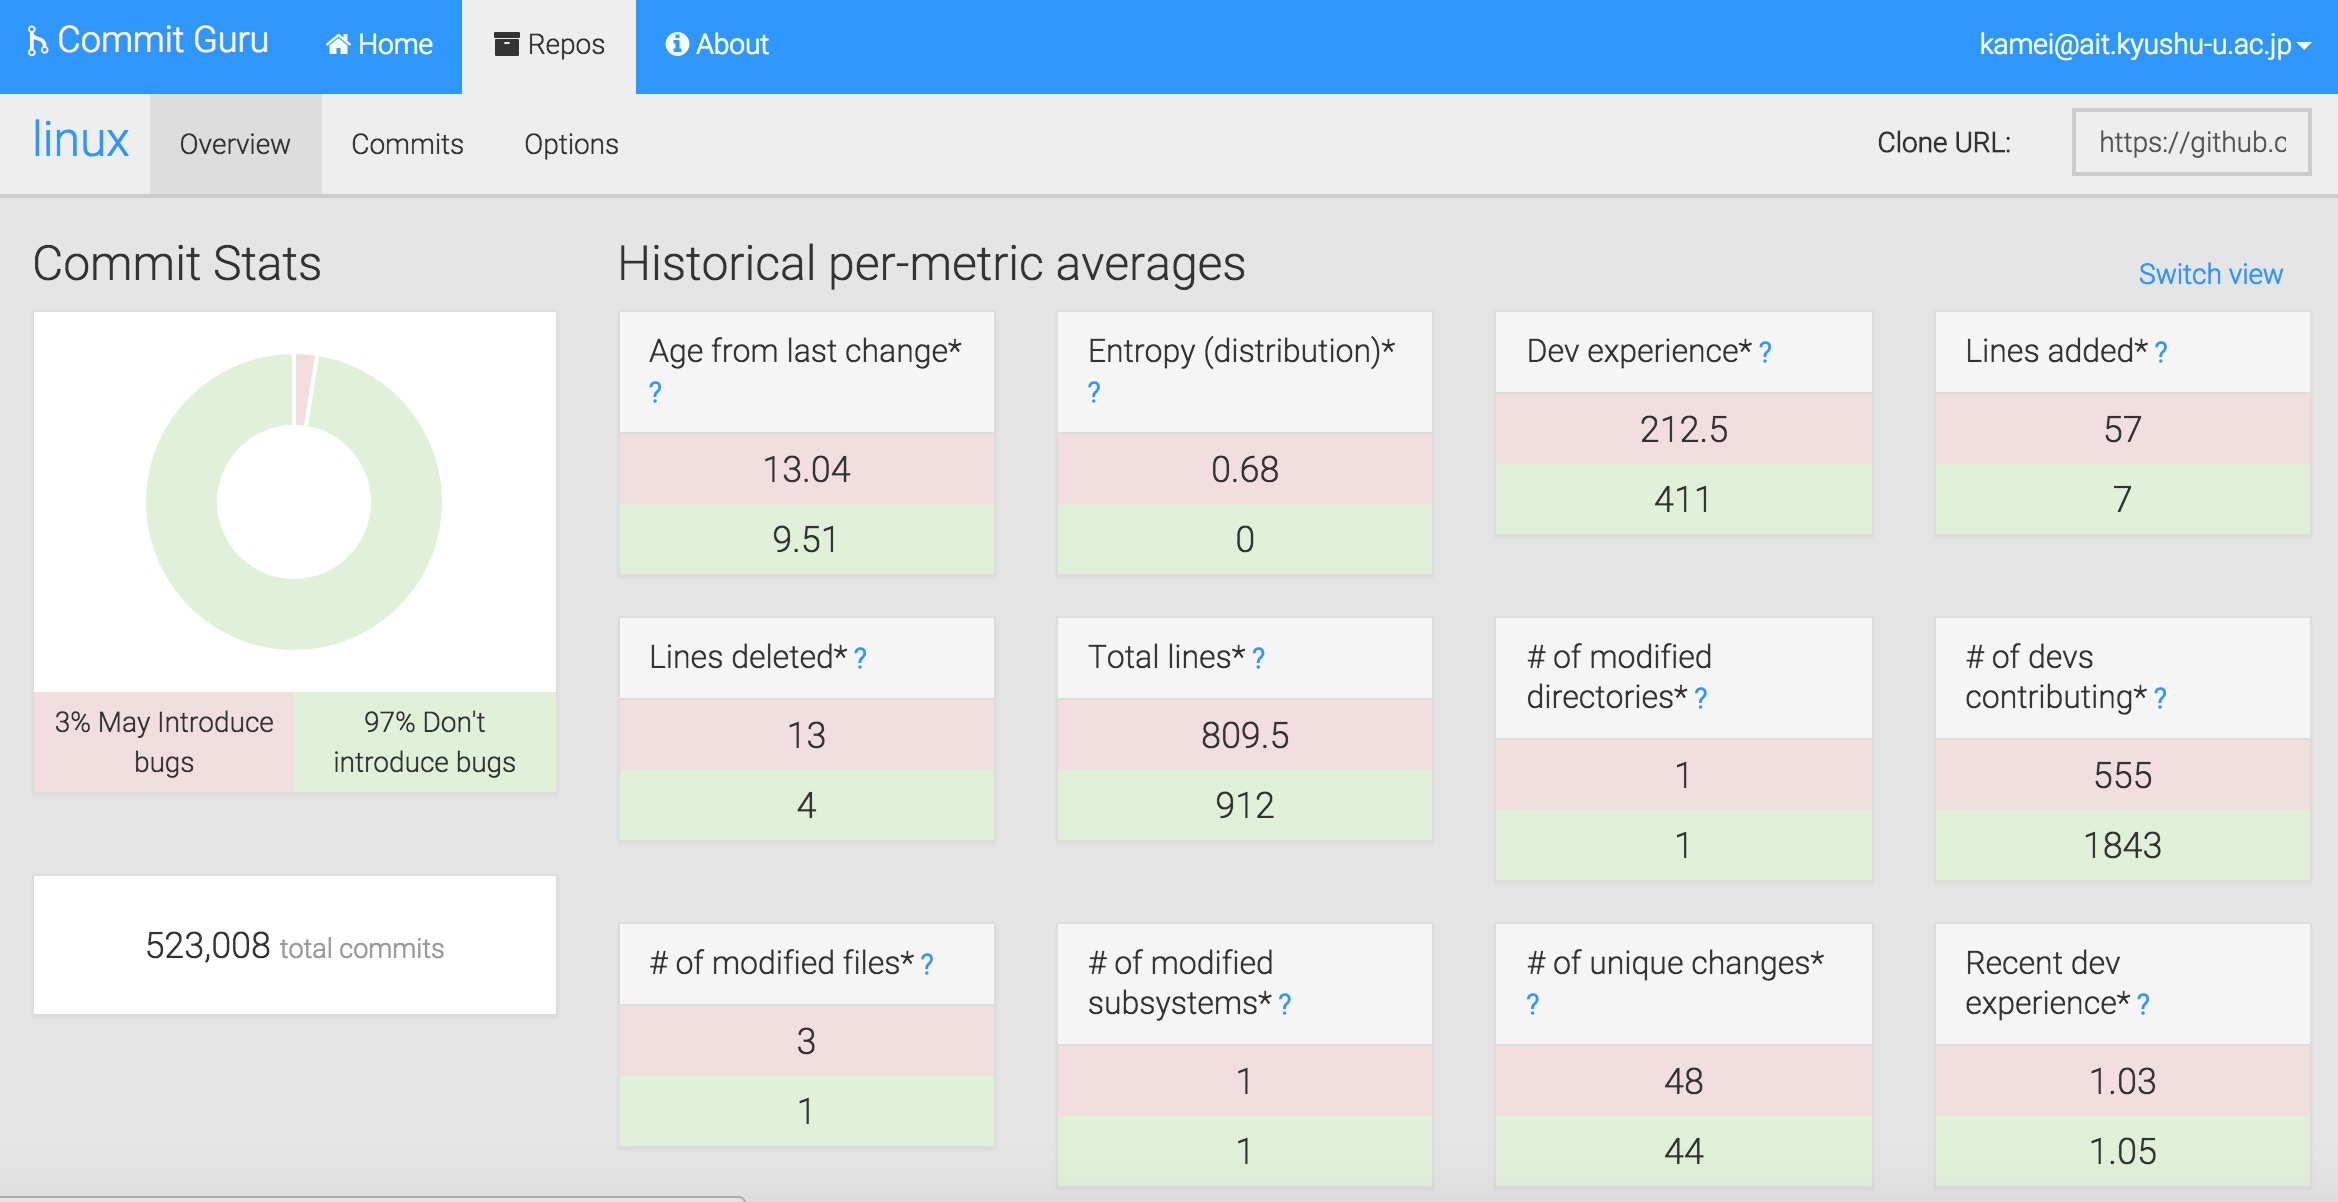
\includegraphics[width=.4\textwidth]{figures/guru2}
  \caption{Commit Statistics in Commit Guru \label{fig:guru2}}
\end{figure}
%-----------------------------------------------------------------------

\smallsection{Future Challenge 4: Knowing How to Fix a Defect!}
The main purpose of defect prediction models thus far has been three-fold: 1) to predict where defects might appear in the future and allocate SQA resources to defect-prone artifacts (e.g., subsystems and files), 2) understand the effect of factors on the likelihood of finding a defect and 3) derive practical guidelines for future software development projects. Although such models have proven to be useful in certain contexts, how to fix the defects that are flagged remains to be an open question.

Therefore, we envision that future defect prediction models will not only predict where the defects are, they will also provide information on how to best fix these defects. For future, we need to understand what kind of defects happen and why such defects happen to give developers more information to locate and fix the predicted defect. One area of research that maybe useful here is the area of automated program repair~\cite{LeGoues2012ICSE, Mechtaev2015ICSE, Nguyen2013ICSE}, which produces candidate patches for validation and deployment, when we obtain the alert of defects from defect prediction models.

%%%%%%%%%%%%%%%%%%%%%%%%%%%%%%%%%%%%%%%%%%%%%%%%%%%%%%%%%%%
\subsection{Model evaluation}

\begin{comment}
\smallsection{Challenge 9: Making our study easy to use and replicate.}

\emad{Yasu, I feel this can be combined with the point above OSS vs. commericla above.}
\Yasu{Emad, I dropped this, because this challenge is similar to trend 1.}
Recently, software engineering research papers have been trying to open their replication packages (e.g., including dataset, tool/script and ReadMe) to re-run their experiments by a third party.
The reason is mainly for (1) showing validity and transparency of the experiments and (2) giving other researchers opportunities to conduct replication studies using other datasets or compare the performance of new models with the original models using same datasets.
In ESEC/FSE 2015~\cite{FSE2015}, which is the flagship conference for Software Engineering, 16 out of 74 papers open such replication packages.\footnote{If the title of papers includes the term ``(with replication package)'', we identify that the papers open their replication packages.} 
While some defect prediction papers also open the replication packages, several papers only describe the approach (e.g., how do they measure the used metrics and how do they build prediction models) and performance (e.g., precision and recall) of the proposed models (i.e., still do not open replication packages). 

If we are interested in the models that papers propose, we want to perform replication studies to generalize the models and to know baseline performance when we propose a new model. 
Such replication studies play an important role for evolving the research field of defect prediction.
However, if we cannot access replication packages, it reduces the speed of such replication studies because we carefully read the paper and need to implement the proposed models ourselves. For future, we will try to open replication packages.
\end{comment}

\smallsection{Future Challenge 5: Simple is Better!}
%This challenge is similar to the previous challenge. While the previous challenge is more related to research interests, this challenge is more related to practical interests. We also need to consider how we simple our proposed models and replication packages are to use. When we just want to use a replication package, some types of replication packages are not suitable: (e.g., we need to carefully read README, set up some environment or modify some scripts to use them due to different environment with the replication packages). In that case, we may give up on using these techniques due to time unless we really would love to use them. We lose many chances that our proposed models are used in practice.

Recently, software engineering research papers have been trying to open their replication packages (e.g., including dataset, tool/script and ReadMe) to re-run their experiments by a third party.
The reason is mainly for (1) showing validity and transparency of the experiments and (2) giving other researchers opportunities to conduct replication studies using other datasets or compare the performance of new models with the original models using same datasets. However, for practice, we need to consider how we simple our proposed models and replication packages are to use. When we just want to use a replication package, some types of replication packages are not suitable: (e.g., we need to carefully read README, set up some environment or modify some scripts to use them due to different environment with the replication packages). In that case, we may give up on using these techniques due to time unless we really would love to use them. We lose many chances that our proposed models are used in practice.

To avoid losing the chances that our proposed models are used in practice, for future of defect prediction models, we should provide simple interface to be used such as web-base interface or virtual image \emad{Should we give simple interfaces or simple models?} \yasu{We should give simple interfaces. Commit guru is very easy to start to use.}.
Furthermore, it would be great by providing the access to our tool via REST-APIs and original scripts for the people who want to integrate the tool into their project. 
For example, Commit Guru~\cite{Rosen2015FSE} provides a language agnostic analytics and prediction tool that identifies and predicts risky software commits (Figure \ref{fig:guru1} and Figure \ref{fig:guru2}).
It is publicity available via web browsers and easy to use. The tools simply requires a URL of a Git repository that you want to analyze (Figure \ref{fig:guru1}).
Its source code is freely available under the MIT license.\footnote{It can be downloaded at \url{https://github.com/
CommitAnalyzingService/CAS_Web} (front-end) and \url{https://github.com/
CommitAnalyzingService/CAS_CodeRepoAnalyzer} (back-end).}
In short, we need to make our tools simple and extendable.

%While we need to spend a lot of effort to make our techniques available through tools that are easy to use, building such tools is likely to be less appreciated than publishing papers \emad{this may be a controversial statement}. We suggest that in the future, the number of the usage/downloads of tools should be considered in the promotion of researchers in the field of defect prediction. 
% \yasu{I agree. I dropped.}

\smallsection{Future Challenge 6: Focusing on Effort}
From the year 2000~\cite{Fenton2000ICSE}, we have one argument that we need to evaluate our prediction models in a practical setting (e.g., how much effort do defect prediction models reduce?) instead of only precision and recall. Recent studies try to tackle such problems when considering effort~\cite{Kamei2010ICSM,Mende2010CSMR}. Such studies use LOC or churn as a proxy for effort.
However, our previous studies~\cite{Shihab2013IST} show that using a combination of LOC, code and complexity metrics provides a better prediction of effort than using LOC alone. For future, we need to tackle what is the best way to measure effort in effort-aware defect prediction models. 
%\emad{dude this is about effort, but the title is perceived quality!!!}

%For user's satisfaction, online marketplaces provide many user's feedback as rating.
%We can make use of the user's feedback for our future study.
